\renewcommand{\appendixname}{Anexos}
\appendix
\chapter{Casos de Uso} \label{appendix:useCase}

\begin{table}[!h]
	\begin{center}
		\begin{tabular}{|c|p{10cm}|}
		\hline \textbf{CU3} & Listar diplomas emitidos \\ 
		\hline \textbf{Actor} & Gestor\\ 
		\hline \textbf{Descripci\'on} & El gestor podr\'a realizar consultas para obtener la lista de diplomas emitidos que cumplen con la parametrizaci\'on establecida. \\ 
		\hline 
		\end{tabular}
		\caption{Caso de uso: Listar diplomas emitidos}
		\label{tab:CU3}
	\end{center}
\end{table}

\begin{table}[!h]
	\begin{center}
		\begin{tabular}{|c|p{10cm}|}
		\hline \textbf{CU4} & Listar diplomas revocados \\ 
		\hline \textbf{Actor} & Gestor\\ 
		\hline \textbf{Descripci\'on} & El gestor podr\'a realizar consultas para obtener la lista de diplomas revocados y sus motivos. \\ 
		\hline 
		\end{tabular}
		\caption{Caso de uso: Listar diplomas revocados}
		\label{tab:CU4}
	\end{center}
\end{table}

\begin{table}[!h]
	\begin{center}
		\begin{tabular}{|c|p{10cm}|}
		\hline \textbf{CU5} & A\~nadir diploma \\ 
		\hline \textbf{Actor} & Gestor\\ 
		\hline \textbf{Descripci\'on} & El gestor podr\' a\~nadir diplomas al sistema, al insertar los metadatos que definen las propiedades del certificado a emitir. \\ 
		\hline 
		\end{tabular}
		\caption{Caso de uso: A\~nadir diploma}
		\label{tab:CU5}
	\end{center}
\end{table}

\begin{table}[t]
	\begin{center}
		\begin{tabular}{|c|p{10cm}|}
		\hline \textbf{CU6} & Revocar diploma \\ 
		\hline \textbf{Actor} & Gestor\\ 
		\hline \textbf{Descripci\'on} & El gestor podr\'a revocar diplomas.\\ 
		\hline 
		\end{tabular}
		\caption{Caso de uso: Revocar diploma}
		\label{tab:CU6}
	\end{center}
\end{table}

%\begin{table}[!]
%	\begin{center}
%		\begin{tabular}{|c|c|p{6cm}|}
%		\hline \textbf{H.U} & \textbf{Nombre} & \textbf{Descripci�n}\\
%		\hline 1 & Conocer t�tulos & Como usuario an�nimo quiero poder conocer los certificados de una persona para poder observar las habilidades y estudios de esa persona. \\
%		\hline 2 & Autentificaci�n & Como usuario gestor quiero poder autenticarme para poder tener acceso al sistema. \\
%		\hline 3 & Cerrar sesi�n & Como usuario gestor quiero poder cerrar la sesi�n actual para poder salir de forma segura del sistema. \\
%		\hline 4 & CRUD de usuarios & Como administrador de sistemas quiero poder crear, leer, modificar y eliminar usuarios del sistema para poder gestionar los usuarios del sistema\\
%		\hline 5 & Crear certificado & Como administrador de certificados quiero poder a�adir nuevos certificados al sistema para poder progresivamente automatizar el proceso de emisi�n de credenciales acad�micas.\\
%		\hline 6 & Validar certificados & Como decano, secretario o rector quiero poder validar los certificados para poder garantizar la validez de la credencial digital emitida por mi Universidad.\\
%		\hline 7 & Revocar certificado & Como gestor de certificados quiero poder revocar los certificados para poder invalidar aquellos certificados que por alguna raz�n ya no son v�lidos.\\
%		\hline 8 & Consultar certificados & Como gestor de certificados, decano, secretario o rector quiero poder consultar los certificados en el sistema seg�n los par�metros introducidos para poder facilitar las operaciones requeridas en el momento.\\
%		\hline 
%		\end{tabular}
%		\caption{Descripci�n de las historias de usuario.}
%		\label{tab:backlog}
%	\end{center}
%\end{table}

\chapter{Historias de Usuario}\label{appendix:useHistory}
\begin{table}[!h]
	\begin{center}
		\begin{tabular}{|c|p{10cm}|}
		\hline \textbf{H.U-4} & CRUD de usuarios \\ 
		\hline \textbf{Usuario} & Gestor con rol de administrador de sistemas \\ 
		\hline \textbf{Descripci\'on} & Como administrador de sistemas quiero poder crear, leer, modificar y eliminar usuarios del sistema para poder gestionar los usuarios del sistema \\ 
		\hline 
		\end{tabular}
		\caption{Historia de Usuario: CRUD de usuarios}
		\label{tab:HU4}
	\end{center}
\end{table}

\begin{table}[!h]
	\begin{center}
		\begin{tabular}{|c|p{10cm}|}
		\hline \textbf{H.U-5} & Crear certificado \\ 
		\hline \textbf{Usuario} & Gestor con rol de administrador de de certificados \\ 
		\hline \textbf{Descripci\'on} & Como administrador de certificados quiero poder a\~nadir nuevos certificados al sistema para poder progresivamente automatizar el proceso de emisi\'on de credenciales acad\'emicas. \\ 
		\hline 
		\end{tabular}
		\caption{Historia de Usuario: Crear certificado}
		\label{tab:HU5}
	\end{center}
\end{table}

\begin{table}[!h]
	\begin{center}
		\begin{tabular}{|c|p{10cm}|}
		\hline \textbf{H.U-6} & Validar certificados \\ 
		\hline \textbf{Usuario} & Gestor con rol de decano, secretario o rector \\ 
		\hline \textbf{Descripci\'on} & Como decano, secretario o rector quiero poder validar los certificados para poder garantizar la validez de la credencial digital emitida por mi Universidad. \\ 
		\hline 
		\end{tabular}
		\caption{Historia de Usuario: Validar certificados}
		\label{tab:HU6}
	\end{center}
\end{table}

\begin{table}[!h]
	\begin{center}
		\begin{tabular}{|c|p{10cm}|}
		\hline \textbf{H.U-7} & Revocar certificado \\ 
		\hline \textbf{Usuario} & Gestor con rol de gestor de certificados \\ 
		\hline \textbf{Descripci\'on} & Como gestor de certificados quiero poder revocar los certificados para poder invalidar aquellos certificados que por alguna raz\'on ya no son v\'alidos. \\ 
		\hline 
		\end{tabular}
		\caption{Historia de Usuario: Revocar certificado}
		\label{tab:HU7}
	\end{center}
\end{table}

\begin{table}[!h]
	\begin{center}
		\begin{tabular}{|c|p{10cm}|}
		\hline \textbf{H.U-8} & Consultar certificados \\ 
		\hline \textbf{Usuario} & Gestor con rol de gestor de certificados, decano, secretario o rector \\ 
		\hline \textbf{Descripci\'on} & Como gestor de certificados, decano, secretario o rector quiero poder consultar los certificados en el sistema seg\'un los par\'ametros introducidos para poder facilitar las operaciones requeridas en el momento. \\ 
		\hline 
		\end{tabular}
		\caption{Historia de Usuario: Consultar certificados}
		\label{tab:HU8}
	\end{center}
\end{table}

\chapter{Im\'agenes de la aplicaci\'on}\label{appendix:images}
\begin{figure}[htbp]
\centering
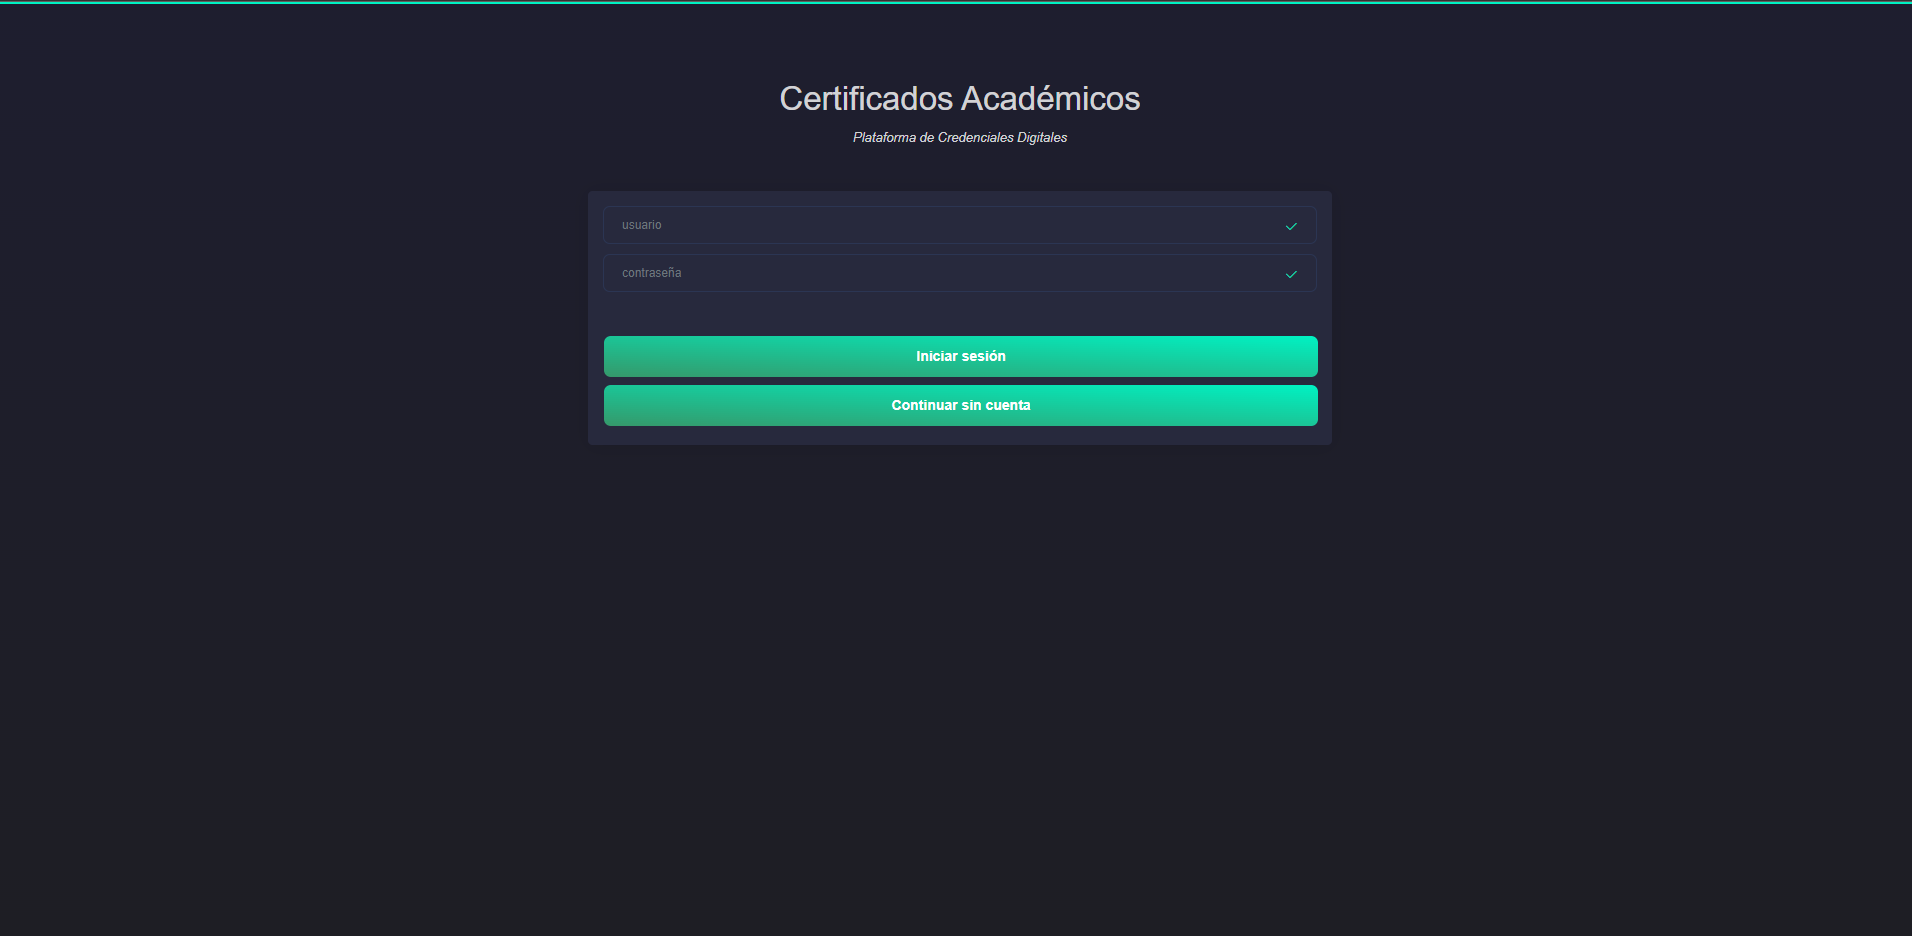
\includegraphics[width=\textwidth]{Graphics/login}
\caption{Vista de iniciar sesi\'on.}
\label{fig:login}
\end{figure}

\begin{figure}[htbp]
\centering
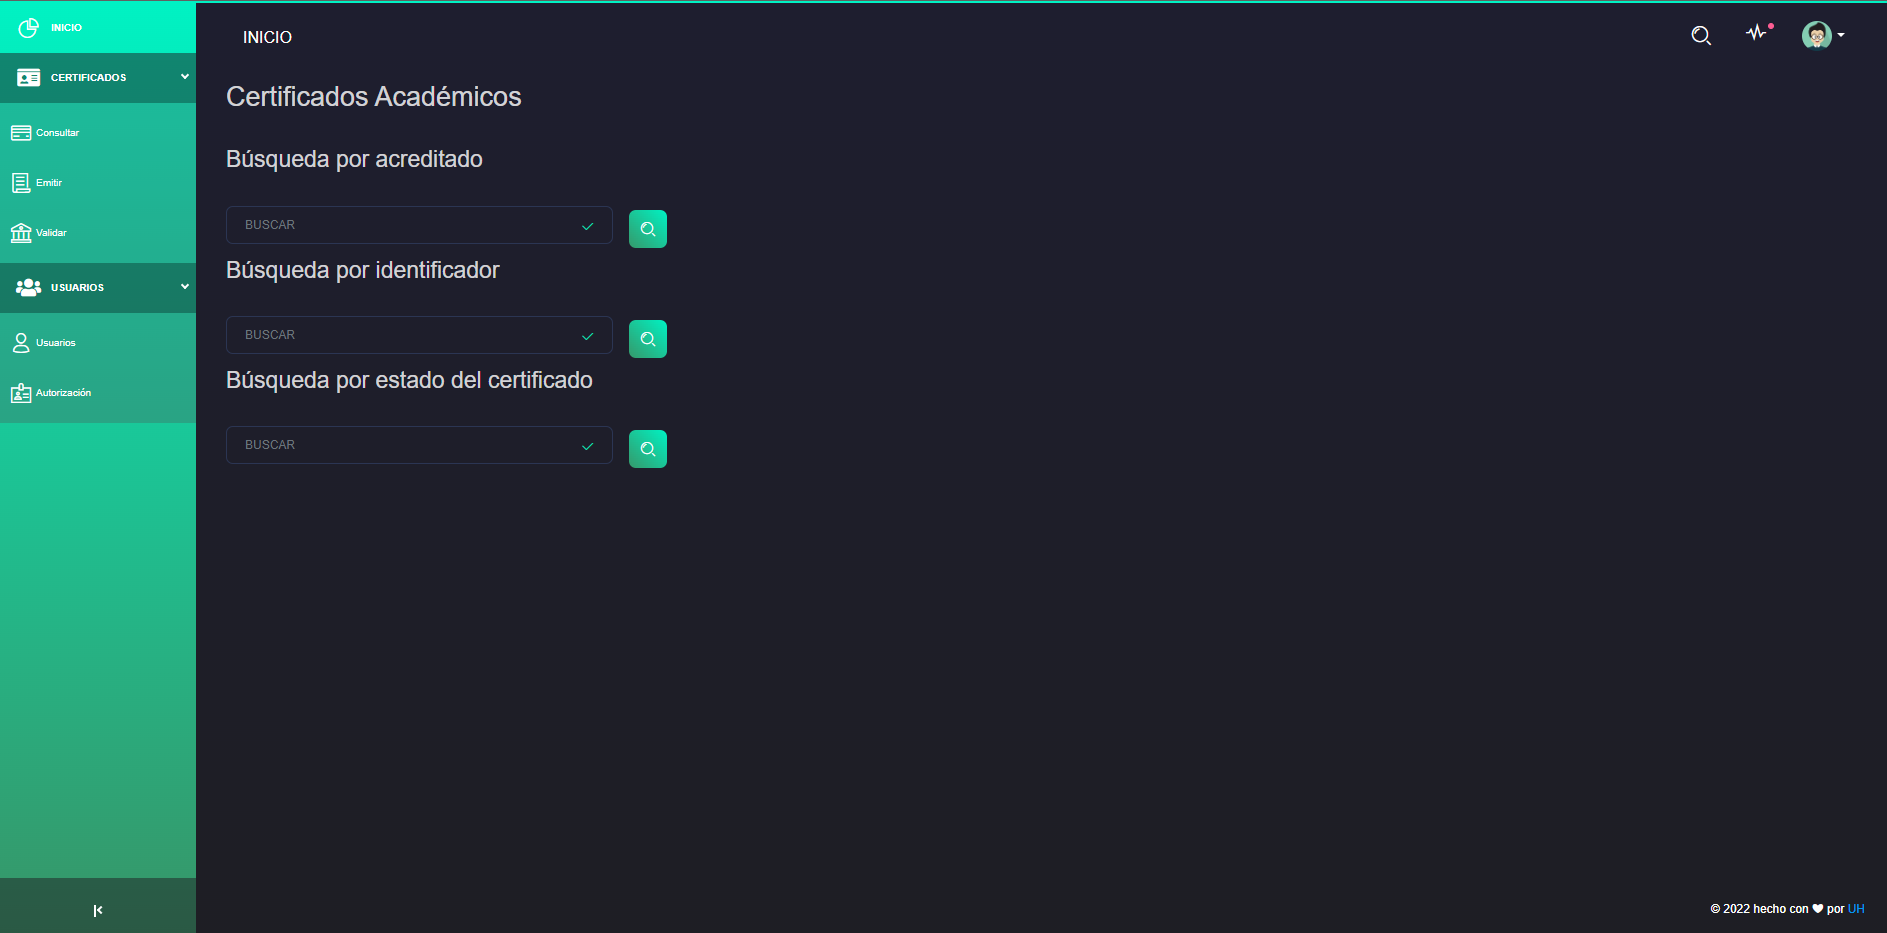
\includegraphics[width=\textwidth]{Graphics/dashboard}
\caption{Vista de inicio.}
\label{fig:dashboard}
\end{figure}

\begin{figure}[htbp]
\centering
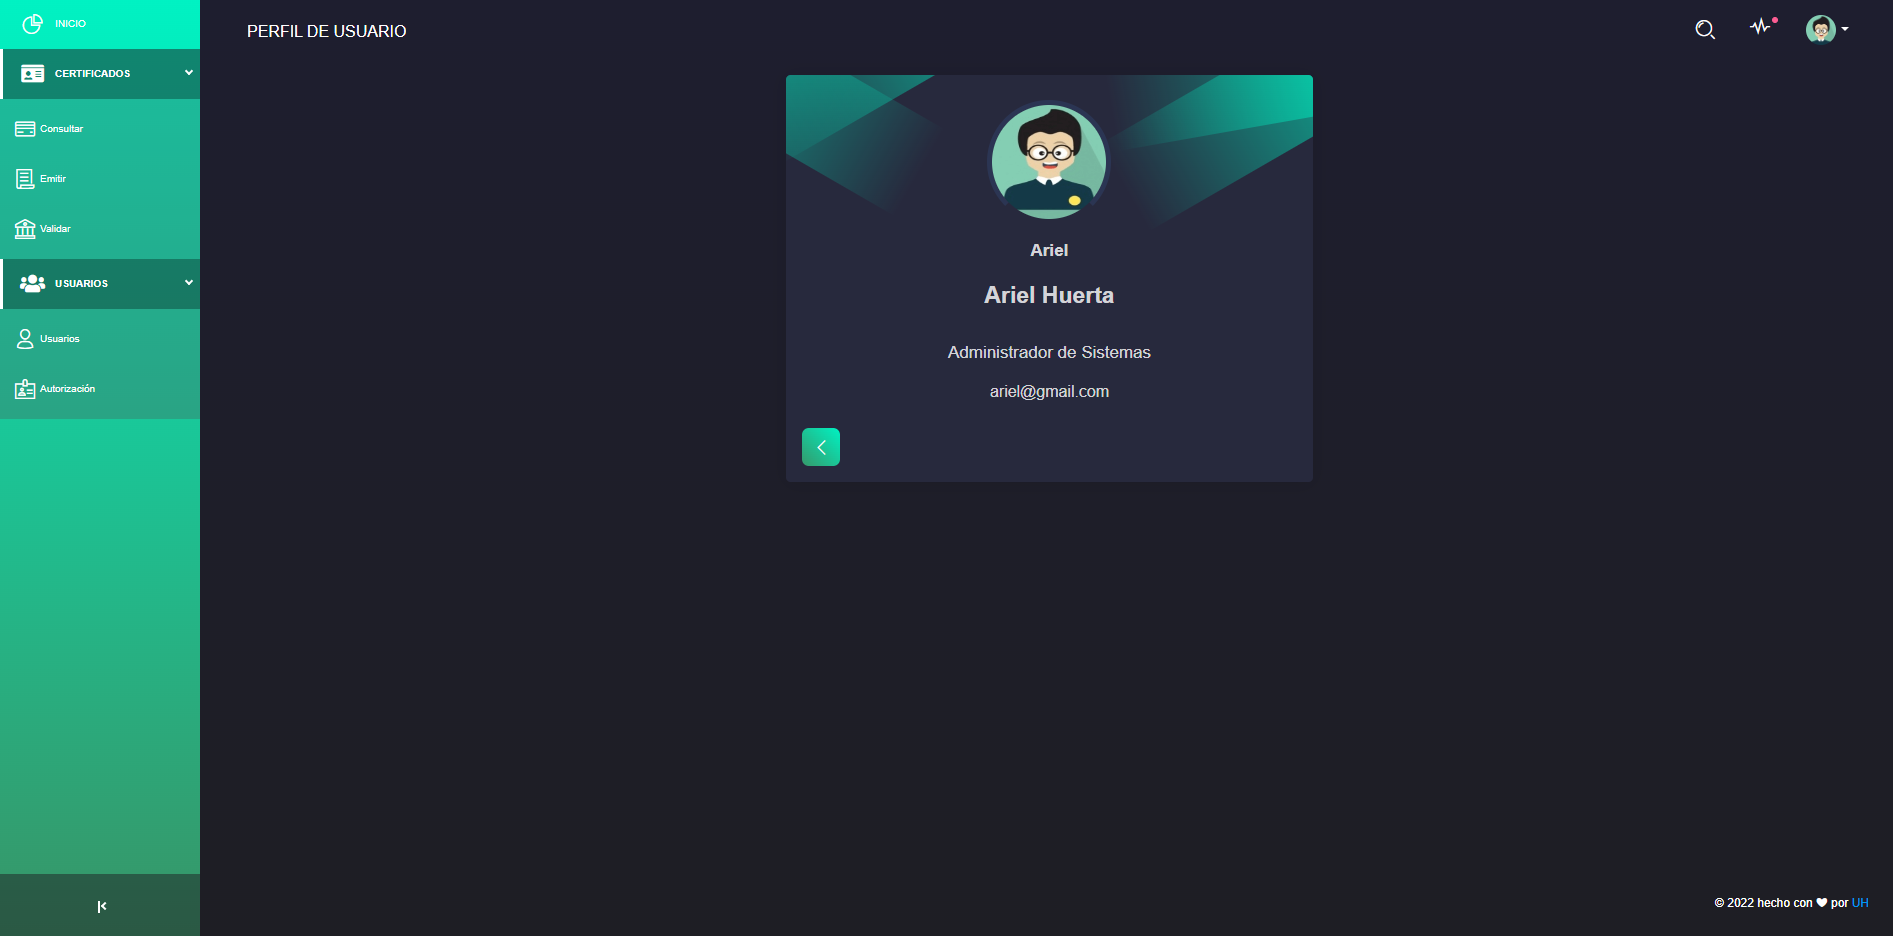
\includegraphics[width=\textwidth]{Graphics/profile}
\caption{Perfil de usuario.}
\label{fig:profile}
\end{figure}

\begin{figure}[htbp]
\centering
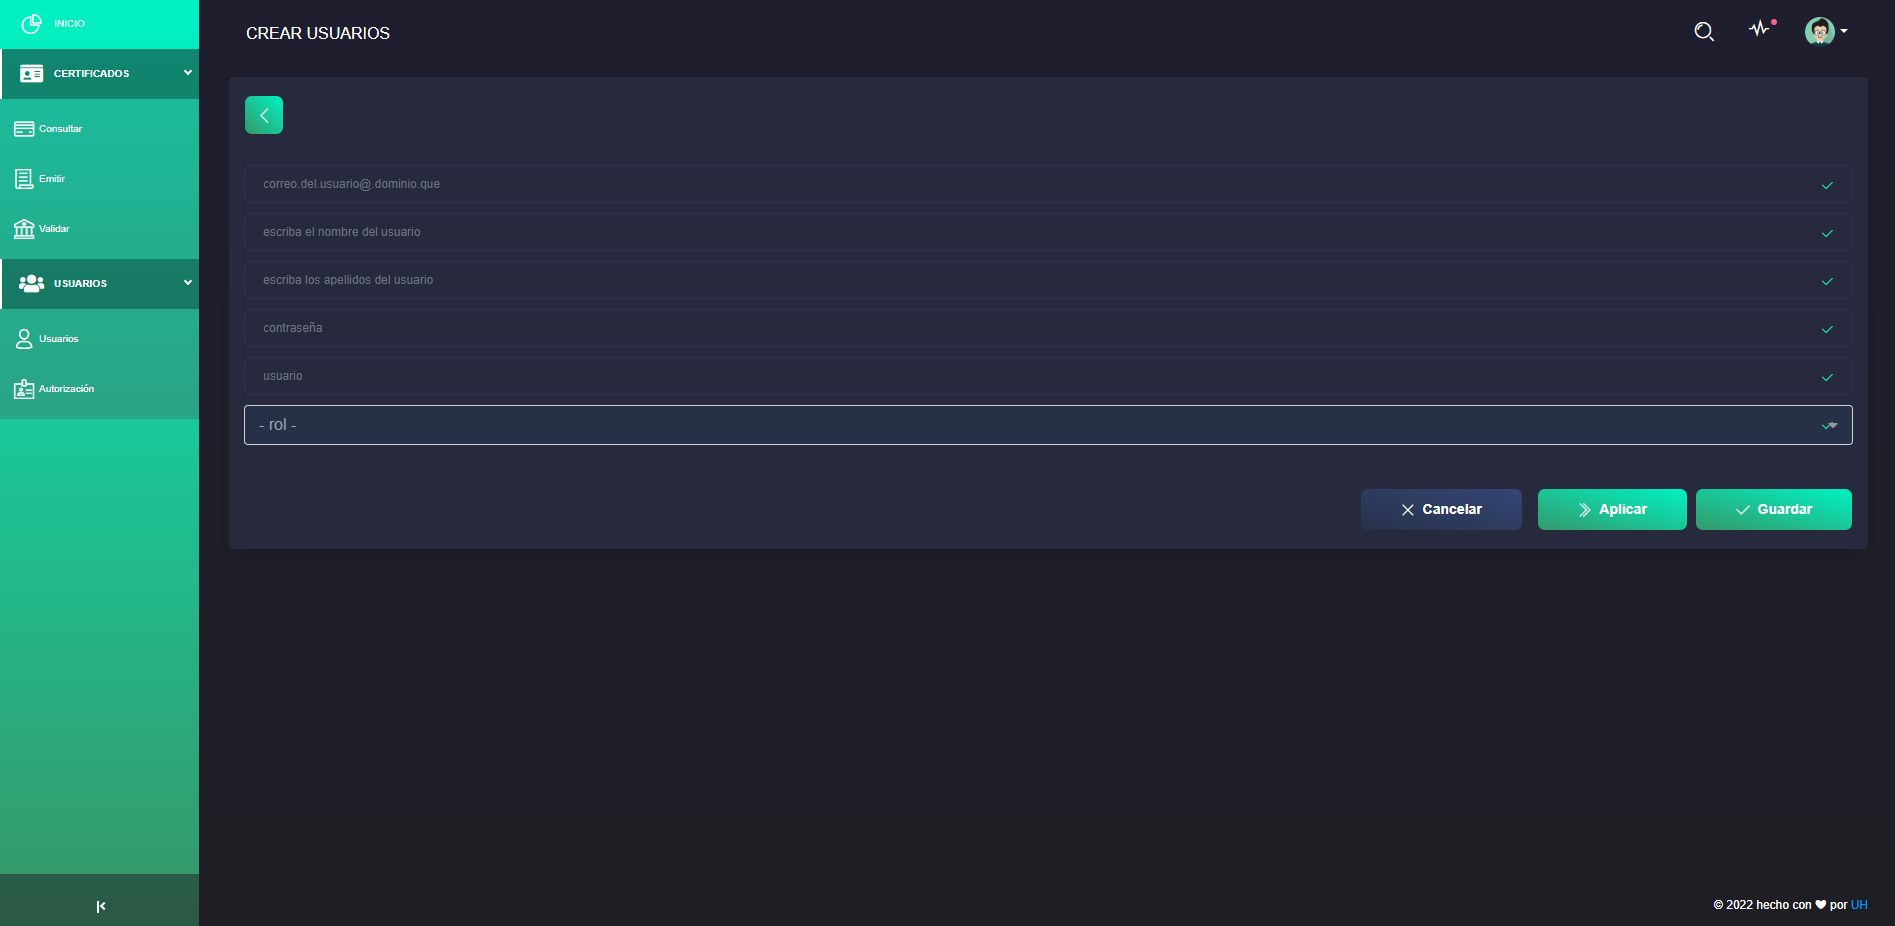
\includegraphics[width=\textwidth]{Graphics/crearusuario}
\caption{P\'agina de crear usuario.}
\label{fig:usercreate}
\end{figure}

\begin{figure}[htbp]
\centering
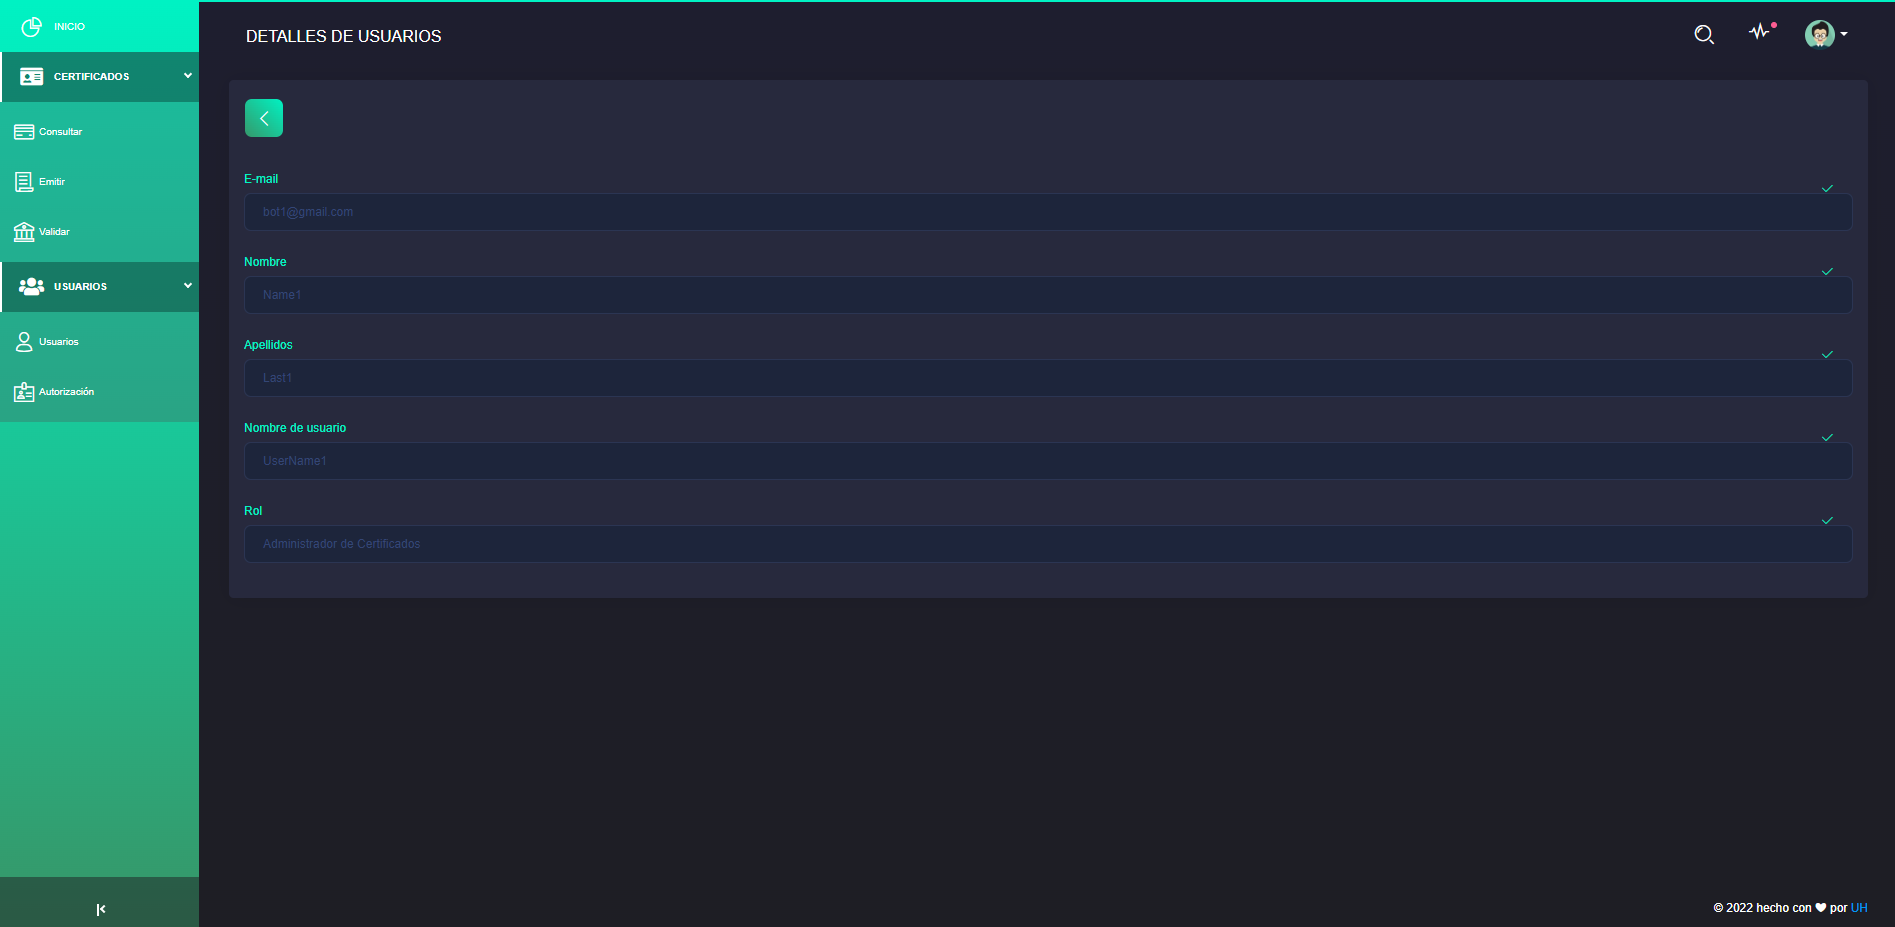
\includegraphics[width=\textwidth]{Graphics/detailsusers}
\caption{P\'agina de detalles del usuario.}
\label{fig:userdetails}
\end{figure}

\begin{figure}[htbp]
\centering
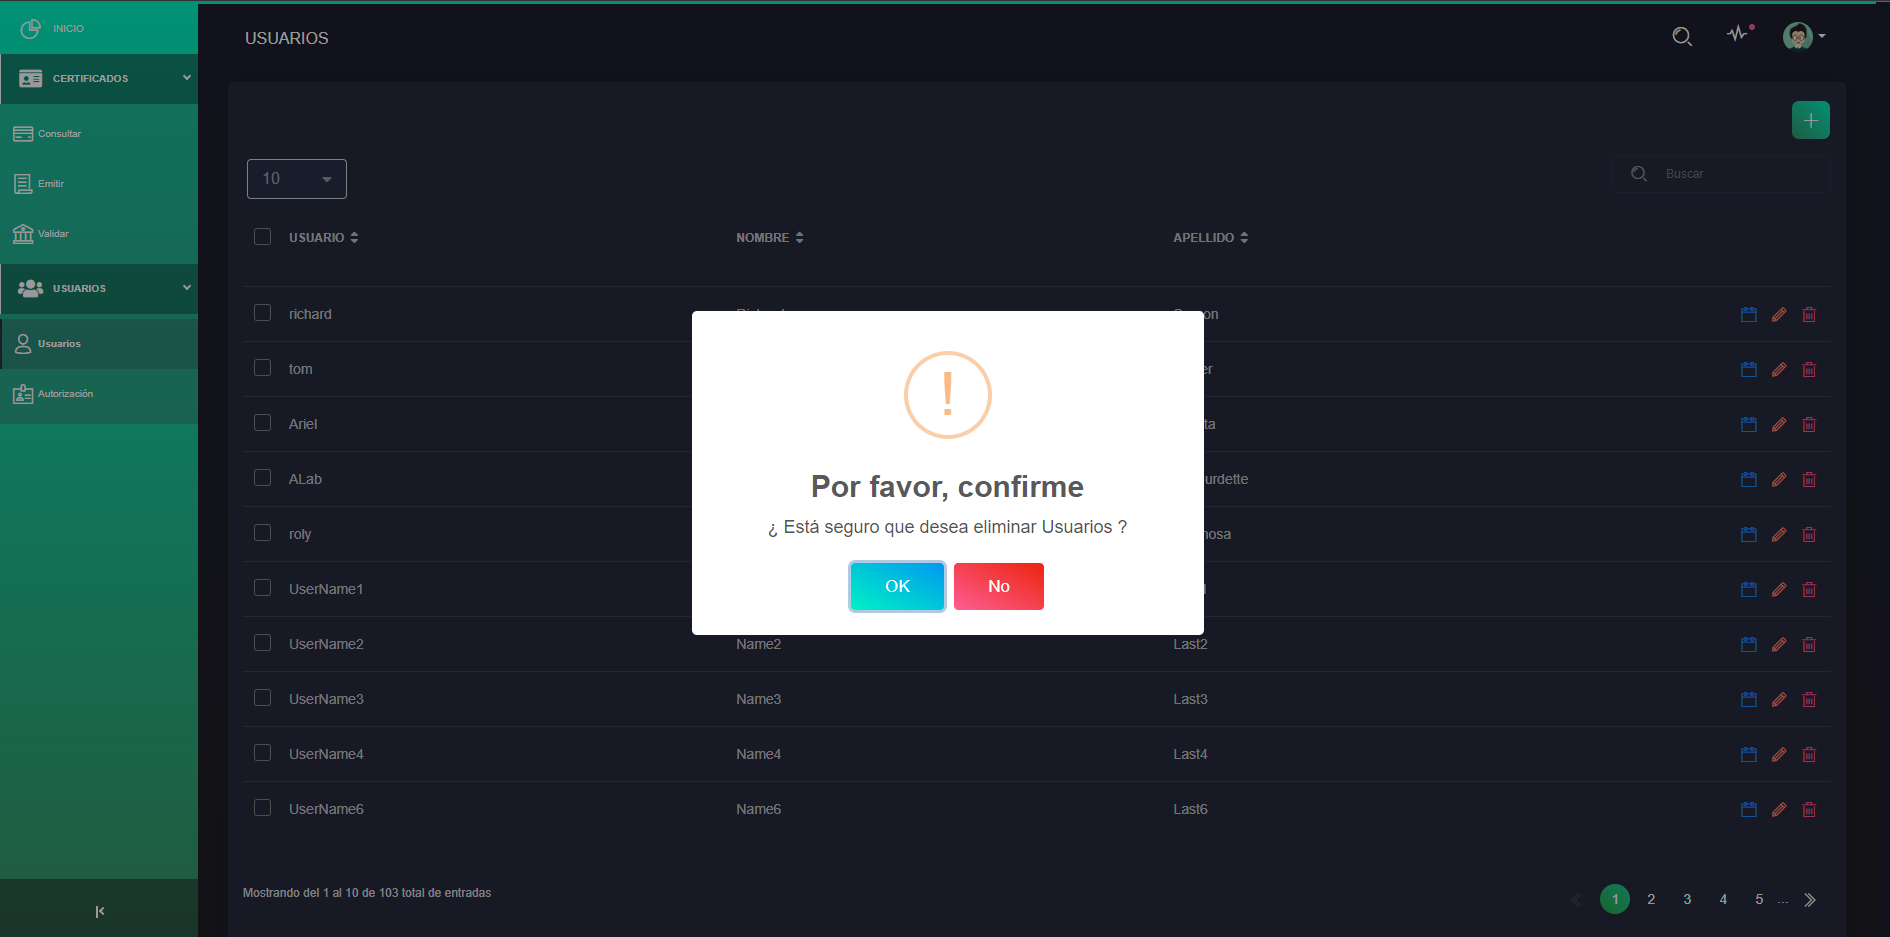
\includegraphics[width=\textwidth]{Graphics/deleteuser}
\caption{Ventana de eliminar usuario.}
\label{fig:userdelete}
\end{figure}

\begin{figure}[htbp]
\centering
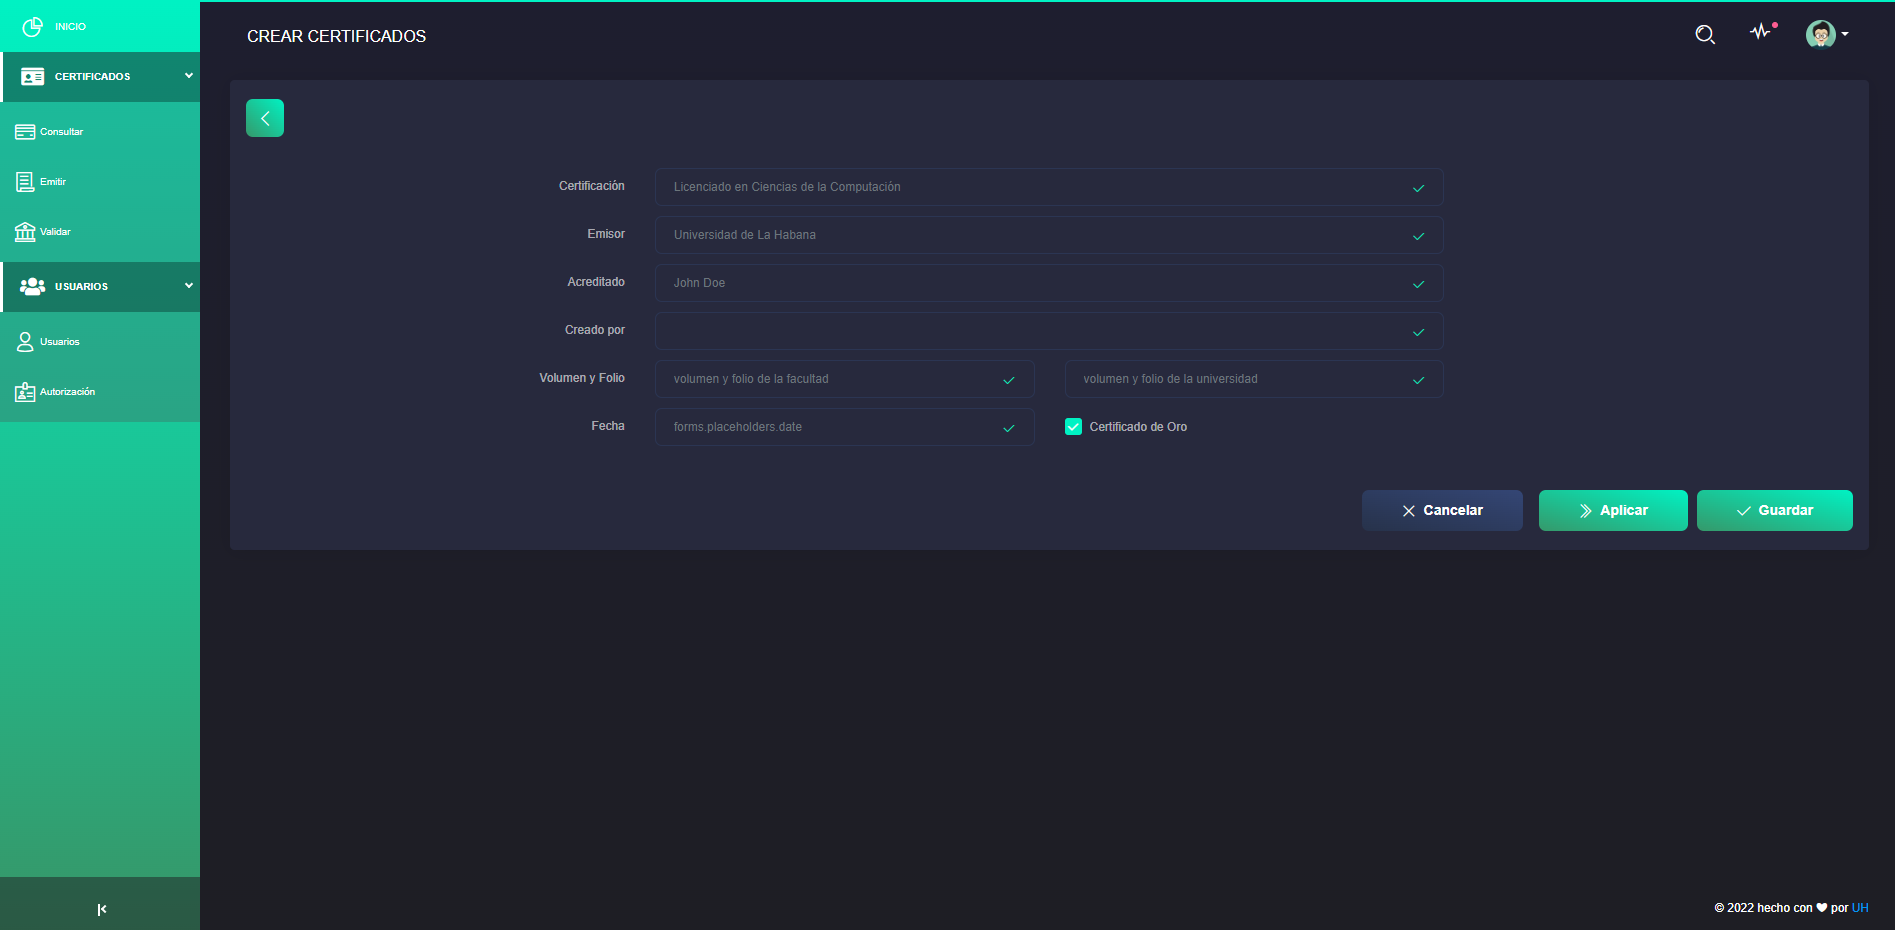
\includegraphics[width=\textwidth]{Graphics/crearcertificados}
\caption{P\'agina de crear certificado.}
\label{fig:usercreate}
\end{figure}

\begin{figure}[htbp]
\centering
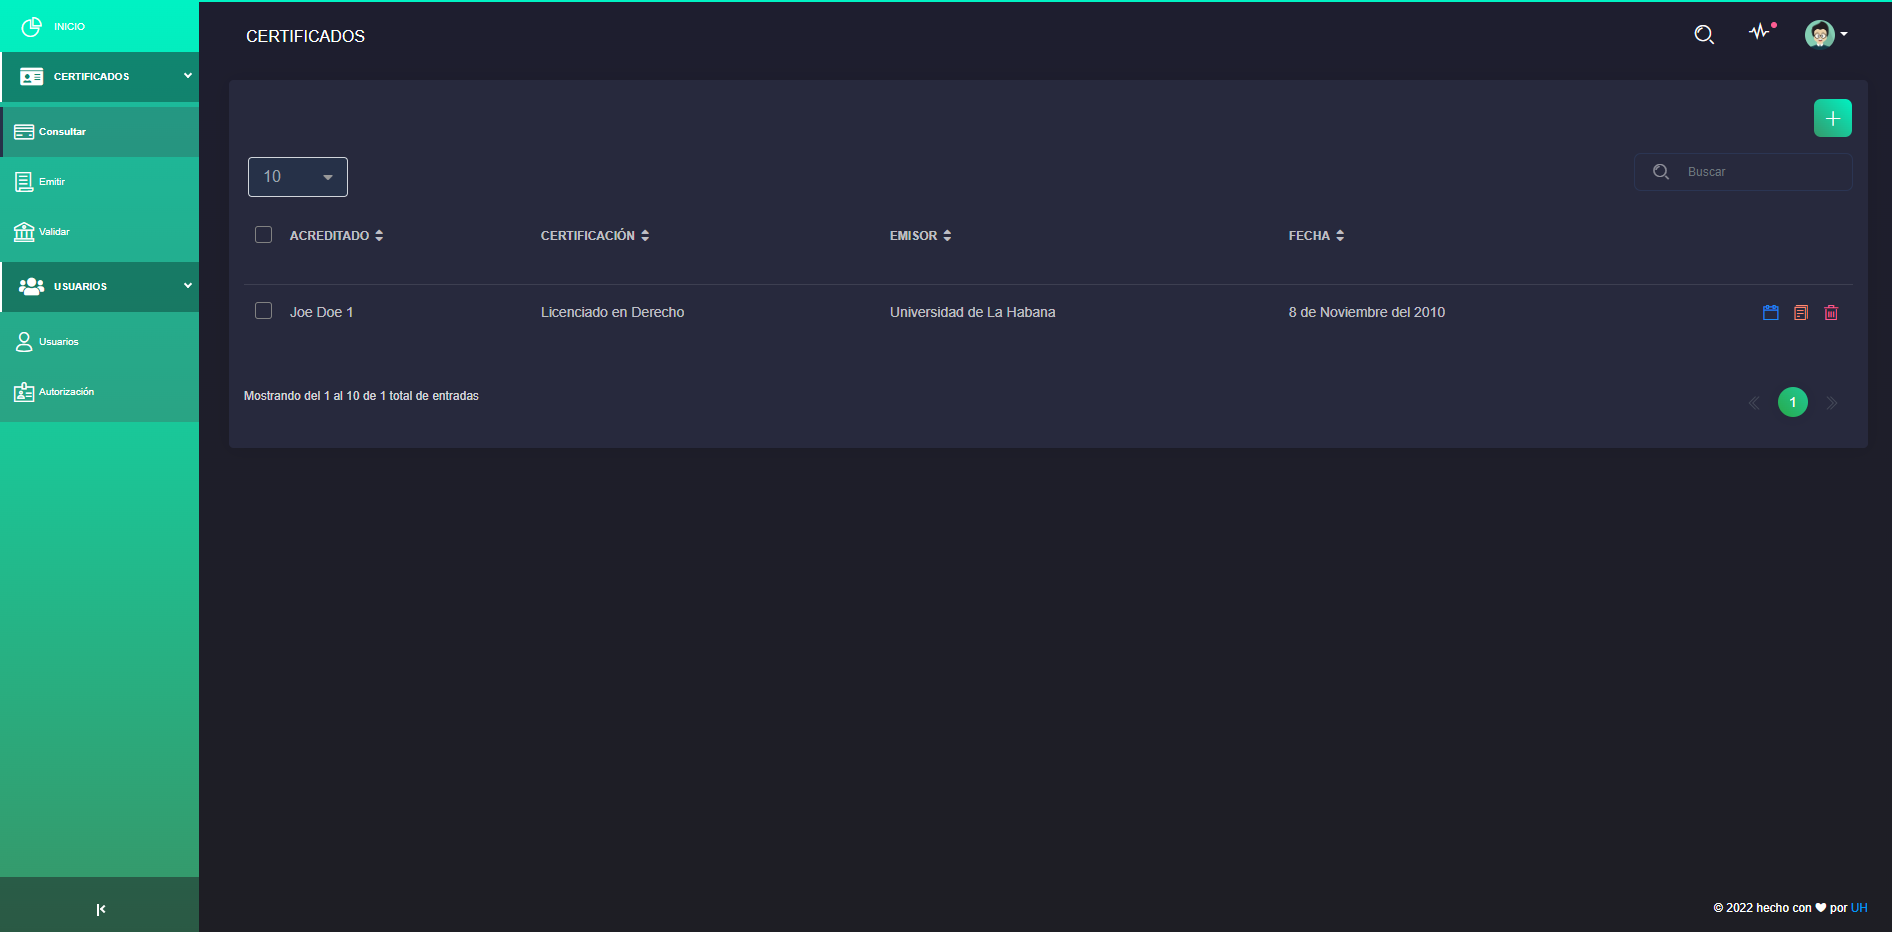
\includegraphics[width=\textwidth]{Graphics/accredited}
\caption{Resultado de una consulta por el nombre del acreditado.}
\label{fig:accredited}
\end{figure}

\begin{figure}[htbp]
\centering
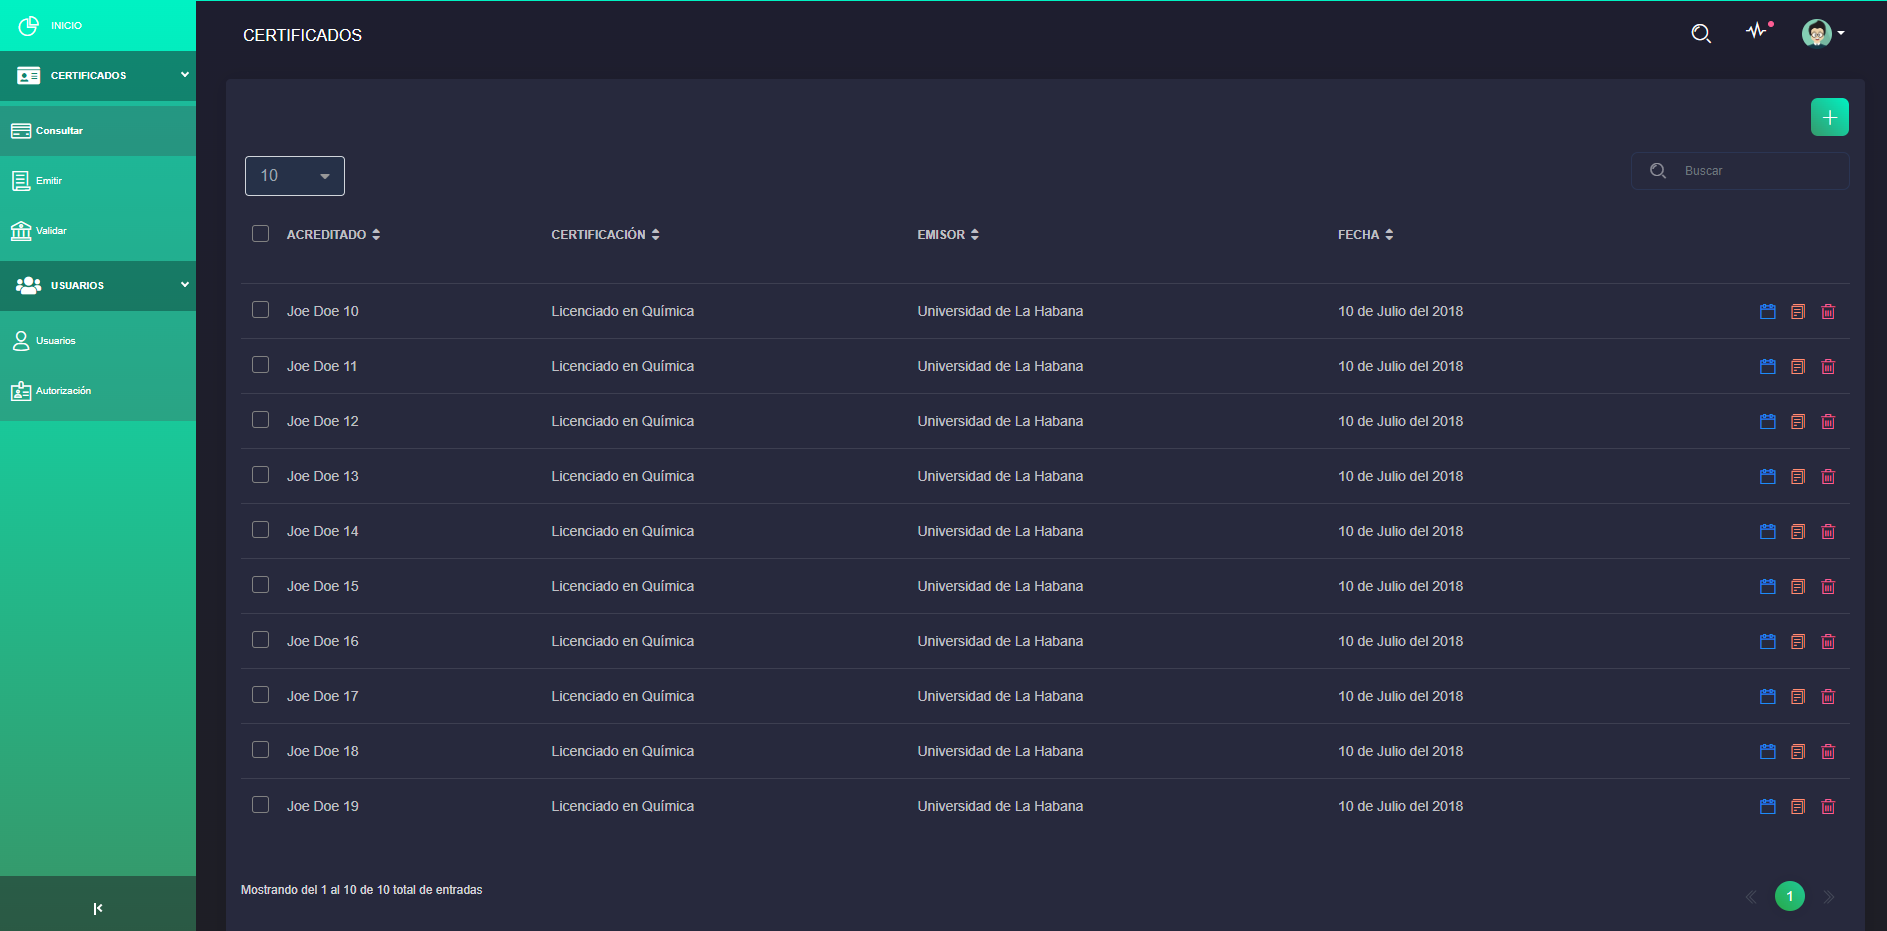
\includegraphics[width=\textwidth]{Graphics/status}
\caption{Resultado de una consulta por el estado del certificado.}
\label{fig:status}
\end{figure}